\documentclass[]{book}
\usepackage{lmodern}
\usepackage{amssymb,amsmath}
\usepackage{ifxetex,ifluatex}
\usepackage{fixltx2e} % provides \textsubscript
\ifnum 0\ifxetex 1\fi\ifluatex 1\fi=0 % if pdftex
  \usepackage[T1]{fontenc}
  \usepackage[utf8]{inputenc}
\else % if luatex or xelatex
  \ifxetex
    \usepackage{mathspec}
  \else
    \usepackage{fontspec}
  \fi
  \defaultfontfeatures{Ligatures=TeX,Scale=MatchLowercase}
\fi
% use upquote if available, for straight quotes in verbatim environments
\IfFileExists{upquote.sty}{\usepackage{upquote}}{}
% use microtype if available
\IfFileExists{microtype.sty}{%
\usepackage{microtype}
\UseMicrotypeSet[protrusion]{basicmath} % disable protrusion for tt fonts
}{}
\usepackage[margin=1in]{geometry}
\usepackage{hyperref}
\hypersetup{unicode=true,
            pdftitle={MARSS wiki},
            pdfauthor={EE Holmes},
            pdfborder={0 0 0},
            breaklinks=true}
\urlstyle{same}  % don't use monospace font for urls
\usepackage{natbib}
\bibliographystyle{apalike}
\usepackage{color}
\usepackage{fancyvrb}
\newcommand{\VerbBar}{|}
\newcommand{\VERB}{\Verb[commandchars=\\\{\}]}
\DefineVerbatimEnvironment{Highlighting}{Verbatim}{commandchars=\\\{\}}
% Add ',fontsize=\small' for more characters per line
\usepackage{framed}
\definecolor{shadecolor}{RGB}{248,248,248}
\newenvironment{Shaded}{\begin{snugshade}}{\end{snugshade}}
\newcommand{\KeywordTok}[1]{\textcolor[rgb]{0.13,0.29,0.53}{\textbf{#1}}}
\newcommand{\DataTypeTok}[1]{\textcolor[rgb]{0.13,0.29,0.53}{#1}}
\newcommand{\DecValTok}[1]{\textcolor[rgb]{0.00,0.00,0.81}{#1}}
\newcommand{\BaseNTok}[1]{\textcolor[rgb]{0.00,0.00,0.81}{#1}}
\newcommand{\FloatTok}[1]{\textcolor[rgb]{0.00,0.00,0.81}{#1}}
\newcommand{\ConstantTok}[1]{\textcolor[rgb]{0.00,0.00,0.00}{#1}}
\newcommand{\CharTok}[1]{\textcolor[rgb]{0.31,0.60,0.02}{#1}}
\newcommand{\SpecialCharTok}[1]{\textcolor[rgb]{0.00,0.00,0.00}{#1}}
\newcommand{\StringTok}[1]{\textcolor[rgb]{0.31,0.60,0.02}{#1}}
\newcommand{\VerbatimStringTok}[1]{\textcolor[rgb]{0.31,0.60,0.02}{#1}}
\newcommand{\SpecialStringTok}[1]{\textcolor[rgb]{0.31,0.60,0.02}{#1}}
\newcommand{\ImportTok}[1]{#1}
\newcommand{\CommentTok}[1]{\textcolor[rgb]{0.56,0.35,0.01}{\textit{#1}}}
\newcommand{\DocumentationTok}[1]{\textcolor[rgb]{0.56,0.35,0.01}{\textbf{\textit{#1}}}}
\newcommand{\AnnotationTok}[1]{\textcolor[rgb]{0.56,0.35,0.01}{\textbf{\textit{#1}}}}
\newcommand{\CommentVarTok}[1]{\textcolor[rgb]{0.56,0.35,0.01}{\textbf{\textit{#1}}}}
\newcommand{\OtherTok}[1]{\textcolor[rgb]{0.56,0.35,0.01}{#1}}
\newcommand{\FunctionTok}[1]{\textcolor[rgb]{0.00,0.00,0.00}{#1}}
\newcommand{\VariableTok}[1]{\textcolor[rgb]{0.00,0.00,0.00}{#1}}
\newcommand{\ControlFlowTok}[1]{\textcolor[rgb]{0.13,0.29,0.53}{\textbf{#1}}}
\newcommand{\OperatorTok}[1]{\textcolor[rgb]{0.81,0.36,0.00}{\textbf{#1}}}
\newcommand{\BuiltInTok}[1]{#1}
\newcommand{\ExtensionTok}[1]{#1}
\newcommand{\PreprocessorTok}[1]{\textcolor[rgb]{0.56,0.35,0.01}{\textit{#1}}}
\newcommand{\AttributeTok}[1]{\textcolor[rgb]{0.77,0.63,0.00}{#1}}
\newcommand{\RegionMarkerTok}[1]{#1}
\newcommand{\InformationTok}[1]{\textcolor[rgb]{0.56,0.35,0.01}{\textbf{\textit{#1}}}}
\newcommand{\WarningTok}[1]{\textcolor[rgb]{0.56,0.35,0.01}{\textbf{\textit{#1}}}}
\newcommand{\AlertTok}[1]{\textcolor[rgb]{0.94,0.16,0.16}{#1}}
\newcommand{\ErrorTok}[1]{\textcolor[rgb]{0.64,0.00,0.00}{\textbf{#1}}}
\newcommand{\NormalTok}[1]{#1}
\usepackage{longtable,booktabs}
\usepackage{graphicx,grffile}
\makeatletter
\def\maxwidth{\ifdim\Gin@nat@width>\linewidth\linewidth\else\Gin@nat@width\fi}
\def\maxheight{\ifdim\Gin@nat@height>\textheight\textheight\else\Gin@nat@height\fi}
\makeatother
% Scale images if necessary, so that they will not overflow the page
% margins by default, and it is still possible to overwrite the defaults
% using explicit options in \includegraphics[width, height, ...]{}
\setkeys{Gin}{width=\maxwidth,height=\maxheight,keepaspectratio}
\IfFileExists{parskip.sty}{%
\usepackage{parskip}
}{% else
\setlength{\parindent}{0pt}
\setlength{\parskip}{6pt plus 2pt minus 1pt}
}
\setlength{\emergencystretch}{3em}  % prevent overfull lines
\providecommand{\tightlist}{%
  \setlength{\itemsep}{0pt}\setlength{\parskip}{0pt}}
\setcounter{secnumdepth}{5}
% Redefines (sub)paragraphs to behave more like sections
\ifx\paragraph\undefined\else
\let\oldparagraph\paragraph
\renewcommand{\paragraph}[1]{\oldparagraph{#1}\mbox{}}
\fi
\ifx\subparagraph\undefined\else
\let\oldsubparagraph\subparagraph
\renewcommand{\subparagraph}[1]{\oldsubparagraph{#1}\mbox{}}
\fi

%%% Use protect on footnotes to avoid problems with footnotes in titles
\let\rmarkdownfootnote\footnote%
\def\footnote{\protect\rmarkdownfootnote}

%%% Change title format to be more compact
\usepackage{titling}

% Create subtitle command for use in maketitle
\newcommand{\subtitle}[1]{
  \posttitle{
    \begin{center}\large#1\end{center}
    }
}

\setlength{\droptitle}{-2em}
  \title{MARSS wiki}
  \pretitle{\vspace{\droptitle}\centering\huge}
  \posttitle{\par}
  \author{EE Holmes}
  \preauthor{\centering\large\emph}
  \postauthor{\par}
  \predate{\centering\large\emph}
  \postdate{\par}
  \date{2018-03-15}

\usepackage{booktabs}
\usepackage{amsthm}
\makeatletter
\def\thm@space@setup{%
  \thm@preskip=8pt plus 2pt minus 4pt
  \thm@postskip=\thm@preskip
}
\makeatother

\begin{document}
\maketitle

{
\setcounter{tocdepth}{1}
\tableofcontents
}
\newcommand{\var}{\mathrm{Var}}

\chapter{Contribute}\label{contribute}

Write an Rmd file. Add via a pull-request.

Each Rmd file contains one and only one entry/vignette. The title of
your vignette must be at the top of your Rmd and have \texttt{\#}
(chapter level). Subsequent headings should be \texttt{\#\#}.

\chapter{Plot states from a DFA using
ggplot}\label{plot-states-from-a-dfa-using-ggplot}

author: EE Holmes date: March 15, 2018

Requires MARSS 3.10.4+

Required packages

\begin{Shaded}
\begin{Highlighting}[]
\KeywordTok{library}\NormalTok{(MARSS)}
\KeywordTok{library}\NormalTok{(broom)}
\KeywordTok{library}\NormalTok{(ggplot2)}
\end{Highlighting}
\end{Shaded}

Load data and zscore

\begin{Shaded}
\begin{Highlighting}[]
\KeywordTok{data}\NormalTok{(lakeWAplankton)}
\CommentTok{# we want lakeWAplanktonTrans, which has been log-transformed}
\CommentTok{# and the 0s replaced with NAs}
\NormalTok{plankdat =}\StringTok{ }\NormalTok{lakeWAplanktonTrans}
\NormalTok{years =}\StringTok{ }\NormalTok{plankdat[,}\StringTok{"Year"}\NormalTok{]}\OperatorTok{>=}\DecValTok{1980} \OperatorTok{&}\StringTok{ }\NormalTok{plankdat[,}\StringTok{"Year"}\NormalTok{]}\OperatorTok{<}\DecValTok{1990}
\NormalTok{phytos =}\StringTok{ }\KeywordTok{c}\NormalTok{(}\StringTok{"Cryptomonas"}\NormalTok{, }\StringTok{"Diatoms"}\NormalTok{, }\StringTok{"Greens"}\NormalTok{,}
                  \StringTok{"Unicells"}\NormalTok{, }\StringTok{"Other.algae"}\NormalTok{)}
\NormalTok{dat.spp.}\DecValTok{1980}\NormalTok{ =}\StringTok{ }\NormalTok{plankdat[years,phytos]}
\CommentTok{# transpose data so time goes across columns}
\NormalTok{dat.spp.}\DecValTok{1980}\NormalTok{ =}\StringTok{ }\KeywordTok{t}\NormalTok{(dat.spp.}\DecValTok{1980}\NormalTok{)}
\NormalTok{dat.z =}\StringTok{ }\KeywordTok{zscore}\NormalTok{(dat.spp.}\DecValTok{1980}\NormalTok{)}
\end{Highlighting}
\end{Shaded}

Fit a DFA with 3 trends. Setting \texttt{maxit} to 50, so it runs fast.

\begin{Shaded}
\begin{Highlighting}[]
\NormalTok{model.list =}\StringTok{ }\KeywordTok{list}\NormalTok{(}\DataTypeTok{m=}\DecValTok{3}\NormalTok{, }\DataTypeTok{R=}\StringTok{"diagonal and unequal"}\NormalTok{)}
\NormalTok{kemz.}\DecValTok{3}\NormalTok{ =}\StringTok{ }\KeywordTok{MARSS}\NormalTok{(dat.spp.}\DecValTok{1980}\NormalTok{, }\DataTypeTok{model=}\NormalTok{model.list,}
    \DataTypeTok{z.score=}\OtherTok{TRUE}\NormalTok{, }\DataTypeTok{form=}\StringTok{"dfa"}\NormalTok{, }\DataTypeTok{control=}\KeywordTok{list}\NormalTok{(}\DataTypeTok{maxit=}\DecValTok{50}\NormalTok{))}
\end{Highlighting}
\end{Shaded}

Make a plot of trends with CIs

\begin{Shaded}
\begin{Highlighting}[]
\KeywordTok{theme_set}\NormalTok{(}\KeywordTok{theme_bw}\NormalTok{())}
\NormalTok{d <-}\StringTok{ }\KeywordTok{tidy}\NormalTok{(kemz.}\DecValTok{3}\NormalTok{, }\DataTypeTok{type=}\StringTok{"states"}\NormalTok{)}
 \KeywordTok{ggplot}\NormalTok{(}\DataTypeTok{data =}\NormalTok{ d) }\OperatorTok{+}\StringTok{ }
\StringTok{   }\KeywordTok{geom_line}\NormalTok{(}\KeywordTok{aes}\NormalTok{(t, estimate)) }\OperatorTok{+}
\StringTok{   }\KeywordTok{geom_ribbon}\NormalTok{(}\KeywordTok{aes}\NormalTok{(}\DataTypeTok{x=}\NormalTok{t, }\DataTypeTok{ymin=}\NormalTok{conf.low, }\DataTypeTok{ymax=}\NormalTok{conf.high), }\DataTypeTok{linetype=}\DecValTok{2}\NormalTok{, }\DataTypeTok{alpha=}\FloatTok{0.1}\NormalTok{) }\OperatorTok{+}
\StringTok{   }\KeywordTok{facet_grid}\NormalTok{(}\OperatorTok{~}\NormalTok{term) }\OperatorTok{+}
\StringTok{   }\KeywordTok{xlab}\NormalTok{(}\StringTok{"Time Step"}\NormalTok{) }\OperatorTok{+}\StringTok{ }\KeywordTok{ylab}\NormalTok{(}\StringTok{"Val"}\NormalTok{)}
\end{Highlighting}
\end{Shaded}

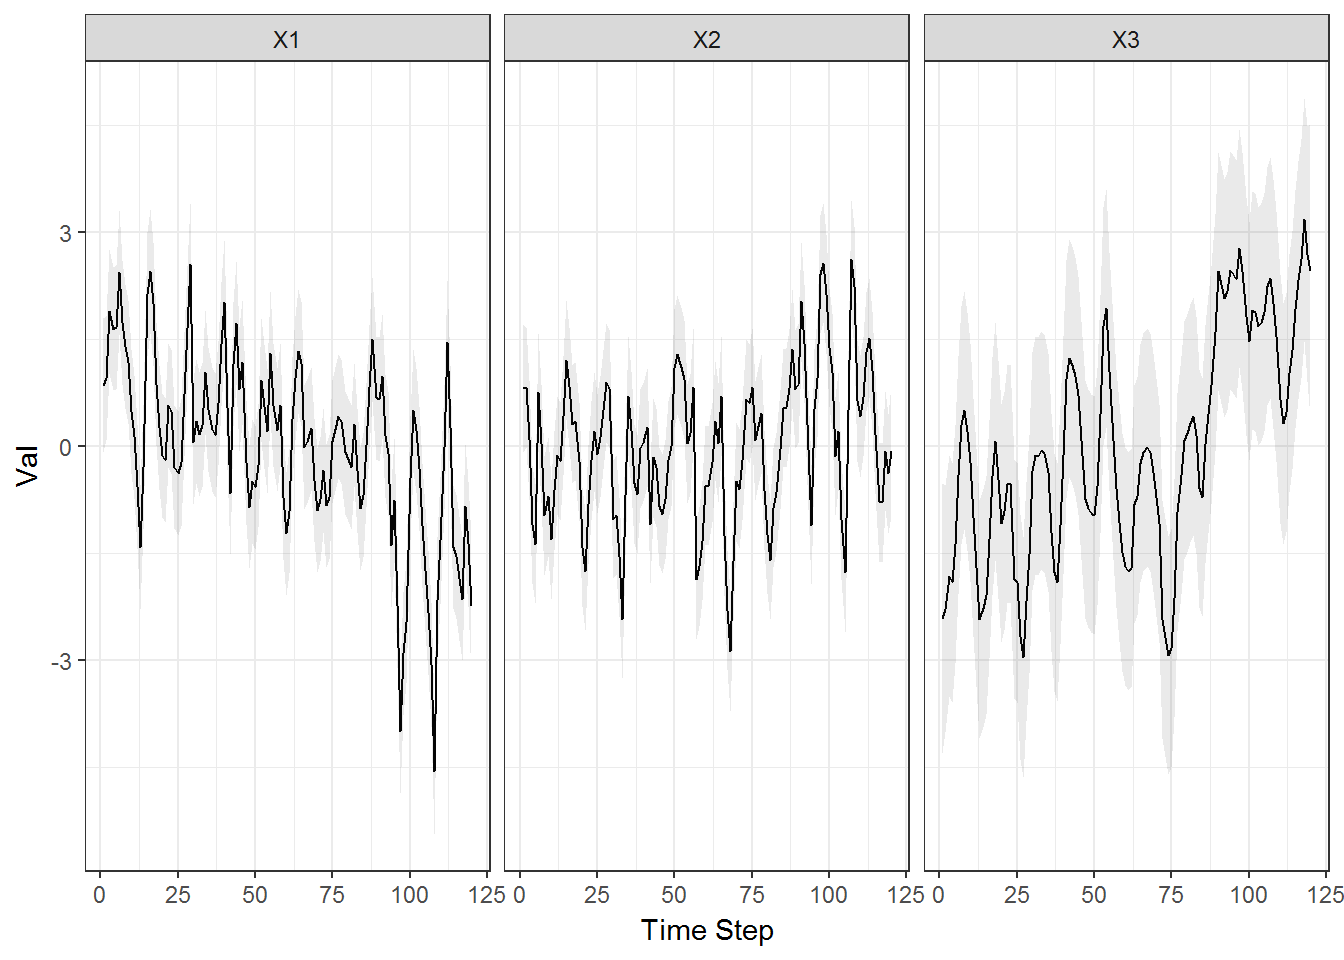
\includegraphics{MARSS-wiki_files/figure-latex/unnamed-chunk-6-1.pdf}

\bibliography{book.bib,packages.bib}


\end{document}
